\section{Preprocessing Top-Level Forms}

Having defined and explained transformation/analyses passes for both patterns and term-templates, these are combined according to the needs of top-level forms. 

Identify three strategies for processing patterns.

NtRewriter -> IdRewriter -> NtCycleChecker -> HoleReachabilitySolver -> AssignableSymbolExtractor for define-language. These accept \lstinline{define-language} form as input and apply described transformations for each pattern in non-terminal definitions.

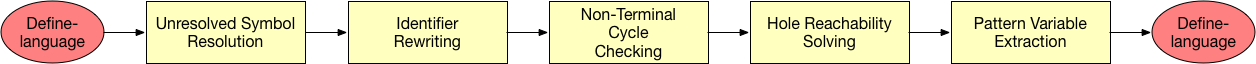
\includegraphics[scale=0.32]{pipeline-pattern-strat-1.png}

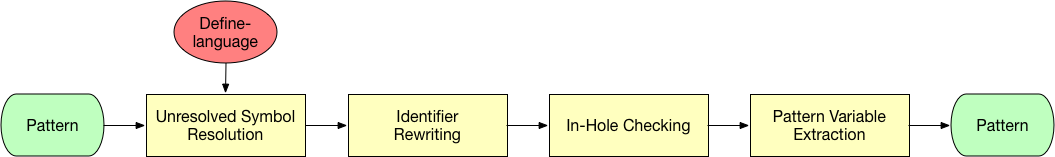
\includegraphics[scale=0.32]{pipeline-pattern-strat-2.png}

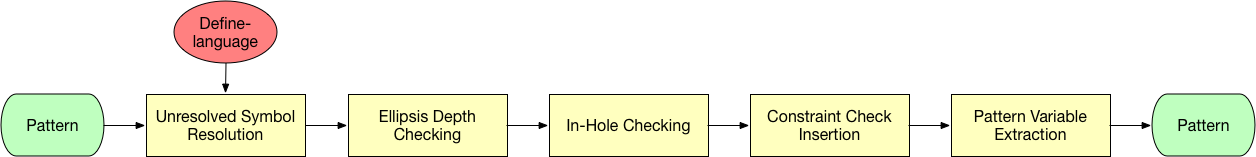
\includegraphics[scale=0.32]{pipeline-pattern-strat-3.png}

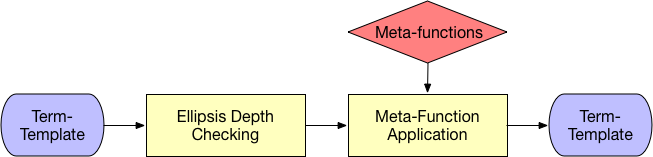
\includegraphics[scale=0.32]{pipeline-term-strat.png}


Notice that non-terminal resolution occurs with respect to some \lstinline{define-language} form. Similarly, during "Metafunction Application Rewriting" pass requires set $Mf$ containing all meta-functions defined until this point. We need to maintain a symbol table for:

\begin{enumerate}
\item All $dl =$ \DefineLanguage forms. Maintain a mapping $L$ that maps $name$ to $dl$
\item All $mf =$ \DefineMetafunction forms. Maintain a mapping $M$ that maps $name$ to $mf$
\item All \lstinline{define-reduction-relation} forms (let it be $r$ and let $n$ be the name of reduction-relation). Maintain a set $R$ that contains $(r, n)$ pairs.
TODO Maintain symbol tables
\end{enumerate}

\subsection{Algorithm}

\begin{itemize}
\item
$d =$ \DefineLanguage 
	\begin{enumerate}
		\item apply strategy (1) to $d$ 
		\item $L = L \cup \{ (name, d) \}$
	\end{enumerate}

\item $m=$ \DefineMetafunction: 
	\begin{enumerate}
	\item Ensure that there exists tuple $(n, d) \in L$ such that $name=n$, otherwise raise Exception.
	\item apply strategy (2) to $domain$ and $codomain$ patterns.
	\item For each $c_i=$ \MetafunctionCase, apply strategy (3) to $p$ and apply term-processing strategy. 
	\item $M = M \cup \{ (name, m) \}$. 
	\end{enumerate}

\item $r=$ \DefineReductionRelation: 
\begin{enumerate}
\item ensure that there exists tuple $(n, d) \in L$ such that $n=languagename$, otherwise raise Exception.
\item Apply strategy (3) to $domain$ pattern. 
\item For each $r_i=$ \ReductionCase in $r$, apply strategy (3) to $p$ and apply the only term-processing strategy. $R = R \cup \{ (name, d) \}$.
\end{enumerate}

\item $tl=$ \ReadFromStdinAndApplyReductionRelation
\begin{enumerate} 
\item If $mf$ is present, ensure there exists tuple $(n, m) \in M$ s.t. $mf=n$, otherwise raise Exception.
\item Ensure there exists tuple $(n, d) \in R$ such that $n=red$, otherwise raise Exception.
\end{enumerate}


\item 
$r=$ \RedexMatchAssertEqual. 
	\begin{enumerate}
	\item Ensure that there exists tuple $(n, d) \in L$ such that $l=n$, otherwise raise Exception.
	\item Process $p$ according to strategy (3). 
	\item Process $t$ according to the only specified strategy.
	\item For each $m=$ \Match, process each $t_i$ according to the only specified strategy.
	\end{enumerate}

\item $tl=$ \TermLetAssertEqual
	\begin{enumerate}
	\item  Process each $t_i$ according to the only specified strategy.
	\item Process $t$ and $e$ according to the only specified strategy.
	\end{enumerate}

\item $tl=$ \ApplyReductionRelationAssertEqual
	\begin{enumerate}
	\item Ensure that there exists tuple $(n, d) \in R$ such that $r=n$, otherwise raise Exception.
	\item Process $t$ according to the only specified strategy.
	\item Process each term $t_i$ according to the only specified strategy.
	\end{enumerate}
\end{itemize}

\subsection{Remarks}
It should be noted that the PyPltRedex handles metafunction resolution is slightly different from PLT Redex. PLT Racket seems to keep track of metafunctions that have been defined up until a certain point, and it also keeps track of metafunctions that have not been defined yet. Roughly speaking, instead of passing a single set $Mf$ into "Metafunction Application Pass", PLT Redex passes a second set $\overline{Mf}$ containing names of metafunctions that haven't been defined yet. This way, when attempting to detect metafunction applications, "Metafunction Application Pass" also checks set $\overline{Mf}$ and raises \lstinline{cannot use metafunction before its definition} error. Since PyPltRedex doesn't handle this, all possible metafunction applications do not get rewritten and thus more often than not $codomain$ check fails.

TODO mention inaccurate treatment of domain checks?
